\documentclass[a4paper,11pt]{report}
\renewcommand{\rmdefault}{phv} %Arial
\renewcommand{\sfdefault}{phv} %Arial
\usepackage[hmargin=2cm,vmargin=2cm, top=2cm, bottom=2cm]{geometry}
\usepackage{hyperref}
\hypersetup{
  colorlinks,
  citecolor=blue
}
\usepackage{color}
\usepackage{bm}
\usepackage{cite}
\usepackage{graphicx}
\usepackage{subfig, float}
\usepackage{verbatim}
\usepackage{minted}
\usepackage{enumitem}


\let\oldbibliography\thebibliography
\renewcommand{\thebibliography}[1]{%
  \oldbibliography{#1}%
  \setlength{\itemsep}{0pt}%
}



\begin{document}


\title{\color{blue}The EINS project: ``Efficient Integrators and
  Non-linear Solvers''}
\author{Alejandro Cosimo}

\maketitle
\tableofcontents

\chapter{Design of the implementation of FETI formulations}

This section gives an overview of the design of the implementation of
FETI formulations in EINS. The design must be general enough in order
to consider different FETI formulations, such as the FETI-1 and
FETI-DP methods. The user must interact with every FETI formulation
through a common interface, from
which the user specifies the type of FETI method to use and the
configuration of the method. If a given option or configuration is
very specific to the considered FETI method, then it is implemented as
a function stating that it is specific to that FETI method, something
like \verb!FETI1SetSometing()!. The following code provides a basic
sketch of how the user would interact with the FETI implementation.


\begin{minted}[frame=lines,framesep=2mm,linenos,mathescape]{c}
  FETI feti;
  FETICreate(comm,&feti);
  FETISetType(feti,FETI1); /*This rutine will call FETICreate_<fetitype>$\label{fetitypeline}$*/
  FETISetMapping(feti, mapping);
  FETISetLocalMatrix(feti,K);
  FETISetLocalRHS(feti,rhs);
  FETISetInterfaceSolver(feti,PJGMRES,PCFETI_DIRICHLET);
  ...
  FETI1SetSometing(feti,...);
  ...
  FETISetFromOptions(feti);
  FETISetUp(feti);/*Here the building of FETI structures takes place*/
  FETISolve(feti,ulocal);/*Solve for the interface problem and obtain ulocal*/
  FETIGetAssmebledSolution(feti,ulocal,ug); /*$\label{globalline}$ulocal is the
  globally unassembled solution, give the user the option to get a vector with
  the assembled solution distributed*/
  FETIGetLambda(pc,lambda); /*Give the user the option to ask for lambda*/
\end{minted}

\noindent Sequence of actions taking place when calling \verb!FETISetUp()!:
\begin{enumerate}[noitemsep,topsep=2pt,parsep=2pt,partopsep=2pt]
\item Build mapping information from local to global DOFs and from
  internal DOFs to boundary DOFs.
\item Build matrices B (if not provided). Also, build information for
  handling the interface problem.
\item Building scaling information.
\item Build intreface problem, that is build \verb!F! and
  \verb!d!. Here, the pseudo-inverse of $\bm{K}$ and the rigid body
  modes are computed.
\item Build KSP and PC for the interface problem.
\item Build projector.
\end{enumerate}

\begin{figure*}[hb]
 \centering
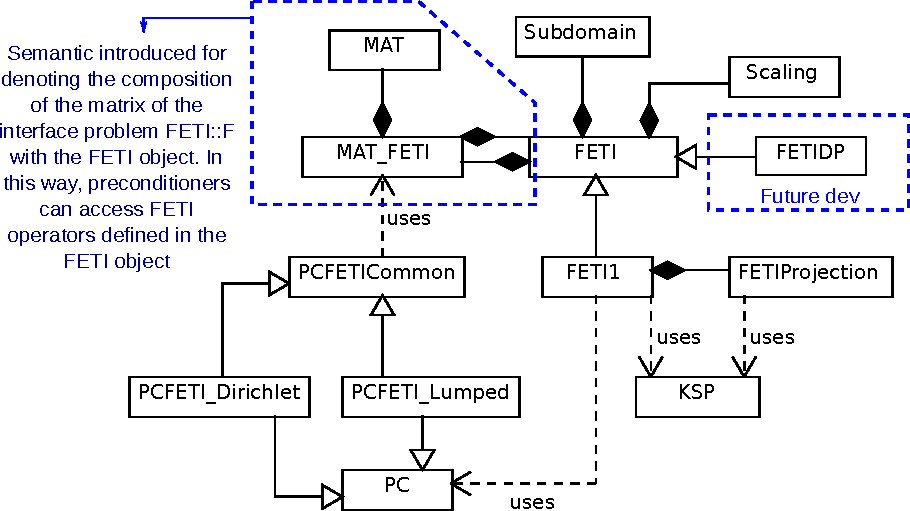
\includegraphics[width=0.8\textwidth]{figures/einsDesign/ClassDiagram.pdf}
\caption{Class diagram of the proposed design.}
\label{fg:classDiagram}
\end{figure*}

\begin{figure*}[hb]
 \centering
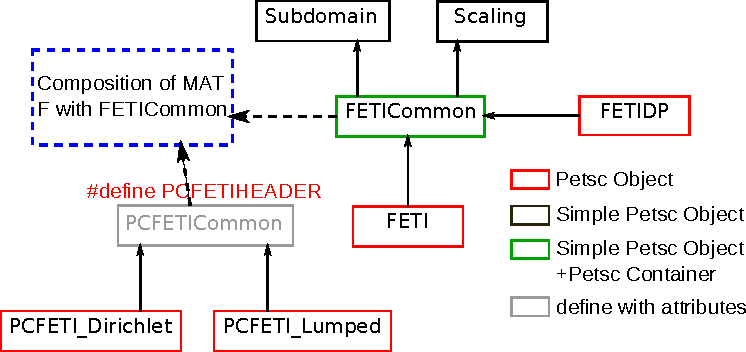
\includegraphics[width=0.8\textwidth]{figures/einsDesign/einsComponents.pdf}
\caption{Details of the implementation of the proposed design. Arrows
  denote dependency between the different classes.}
\label{fg:einsComponents}
\end{figure*}


\begin{figure}[h]
\centering
\subfloat[Detail of the Subdomain class]{
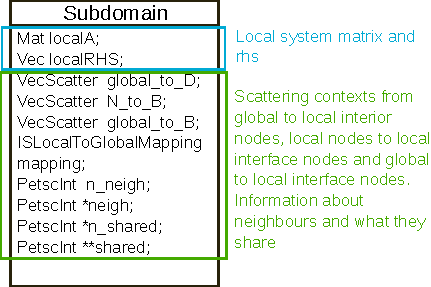
\includegraphics[width=0.45\textwidth]{figures/einsDesign/einsSubdomain.pdf}
\label{fg:einsSubdomain}}~ ~
\subfloat[Detail of the FETI class]{
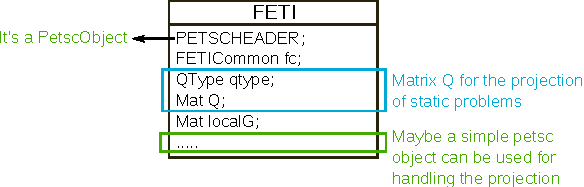
\includegraphics[width=0.5\textwidth]{figures/einsDesign/einsFETI.pdf}
\label{fg:einsFETI}}
\qquad
\subfloat[Detail of the FETI1 class]{
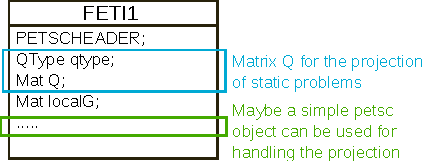
\includegraphics[width=0.45\textwidth]{figures/einsDesign/einsFETI1.pdf}
\label{fg:einsFETI1}}~ ~
\subfloat[Detail of the FETI class]{
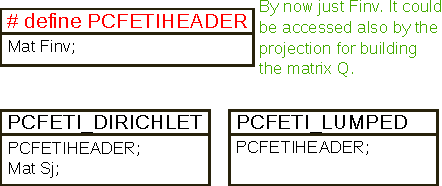
\includegraphics[width=0.45\textwidth]{figures/einsDesign/einsPrecond.pdf}
\label{fg:einsPrecond}}
\caption{Details of the main classes.}
\label{fg:detailsStructures}
\end{figure}


\section{Design of class Subdomain regarding VecScatters}
PETSc VecScatters are objects for managing the communication between
vectors that in general can be sequential or parallel. This is very
useful in DD methods when we need to map a vector to the boundary of
the domain over which it is defined.

For creating a VecScatter two vectors with corresponding indices
for performing the scatter operation (IS objects) must be
provided. The created VecScatter can be used on vectors different from
the ones used for creating the VecScatter, but they must have the same
parallelLayout. For DD method mainly three VecScatters will be useful:

\begin{enumerate}[noitemsep,topsep=2pt,parsep=2pt,partopsep=2pt]
\item \verb!N_to_B!: scattering context from all local nodes to local interface nodes. 
\item \verb!global_to_D!: scattering context from global to local interior nodes.
\item \verb!global_to_B!: scattering context from global to local interface nodes.
\end{enumerate}

The first scatter will be created when calling the function
\verb!SubdomainSetUp()!. This VecScatter is created using the vectors
\verb!vec1_N! and \verb!vec1_B!. If you need to create vectors which
can use the VecScatter \verb!N_to_B!, you can just directly duplicate
the vector \verb!vec1_N! or \verb!vec1_B! by calling to
\verb!VecDuplicate()!.

VecScatters \verb!global_to_D! and \verb!global_to_B! will be not
created by \verb!SubdomainSetUp()!. If you want them to be created,
you must call to \verb!SubdomainCreateVecScatters()! with a reference
to the global vector to be involved by the scatters. A reference to
the global vector provided by the user will be kept in the object
Subdomain in the vector \verb!vec1_global!. In order to build the
VecScatter \verb!global_to_D! the vector \verb!vec1_D! will be
internally used, and it can be used by the user to build extra work
vectors with the ability of performing VecScatters using
\verb!global_to_D! with vectors different from those used for creating
it.




\chapter{Some notes for developers}

\section{Style guide}

The style guides proposed by the PETSc project will be adopted in this
project. People interested in collaborating with the EINS project
should first take a look to the PETSc Developers Manual
\cite{petsc-dev}.

The EINS project relies on the \verb!doctext! tool for producing the
documentation of the code. Please, havea look to the User's manual for
doctext \cite{doctext} in order to correctly document the code. For
each documented function a level of difficulty is specified following
the PETSc convention for that purpose, that is:  
\begin{itemize}[noitemsep,topsep=2pt,parsep=2pt,partopsep=2pt]
\item Beginner - Basic usage
\item Intermediate - Setting options for algorithms and data structures
\item Advanced - Setting more advanced options and customization
\item Developer - Interfaces intended primarily for library developers
\end{itemize}

\section{The git EINS repository}

Good practices for the version control of the EINS project:
\begin{itemize}
\item Avoid placing ignore rules in the local \verb!.gitignore! file
  that only apply to you. For example, if you build your cmake
  project in a directory named \verb!${EINS_DIR}/buildEins!, you don't
  add the ignore rule in the \verb!.gitignore! file from the EINS
  project, but you include that rule in your global \verb!.gitignore_global!
  file. In order to set up your global \verb!.gitignore_global! file, first
  create that file, for example in your home directory, and then type
  \mint{bash}!git config --global core.excludesfile ~/.gitignore_global!
\end{itemize}



\chapter{CMake project implementation}

\section{Basic description of the CMake project}

The scope of the entire cmake project is the one of the current main
CMakeLists file, so some tips:

\begin{itemize}
\item Avoid using \verb!add_subdirectory! and instead use
  \verb!include!. The include command does not change the current
  scope. The \verb!add_directory! changes the scope to the added
  directory.
\item Each target will be defined by the variable \verb!targetName!
  and in general any property will be identified by
  \verb!targetName_property!
\end{itemize}

\noindent Some rules to follow for the implementation of the CMake project:

\begin{itemize}
\item CMake commands are lowercase, e.g. \verb!cmake_minimum_required()!.
\item User macros are uppercase and begin with \verb!M!, e.g. \verb!M_DO_IT()!.
\item User functions are lowercase without the character \verb!_! between
  capitalized words, e.g. \verb!addResource()!.
\item Use macros only where estrictly necessary.  
\end{itemize}

\section{Basic description of the CTest project}

In order to make easier the process of developing stable code, you can
incorporate tests to EINS. For that, you will have to following steps:

\begin{enumerate}
\item Code your test and place it in \verb!${EINS_DIR}/test!. You can
  use the petsc function \verb!SETERRQ! to raice an error in case the
  test is not passed. CTest considers that the test run
  successfully only if it returns ``0''.  
\item Include the test to the EINS CMake project by modifying the file
  \verb!${EINS_DIR}/test/CMakeLists.txt!. Use the macro
  \verb!M_ADD_TEST! whose parameter are the test file and the command
  to run that test. For example:
  \mint{cmake}!M_ADD_TEST("${path}/test.c" "mpiexec -n 4 ./test")!
\item Add a brief description of the test by creating a file with the
  same name of the source code of the test and with the extension
  \verb!rst!, that is like \verb!<TestName>.rst!. For writing the
  content of this file use the
  \href{https://en.wikipedia.org/wiki/ReStructuredText}{ReStructuredText}
  markup features.
\end{enumerate}




\section{Helpful resources for extending the CMake implementation}

\begin{itemize}
\item \href{http://www.cmake.org/Wiki/CMake_FAQ}{Cmake FAQ}
\item \href{http://www.cmake.org/cmake/help/v3.0/command/set_target_properties.html}{Properties definition}
\item \href{http://www.swig.org/Doc1.3/Introduction.html}{SWIG Introduction}
\item
  \href{http://www.cmake.org/Wiki/CMake\%3aCPackConfiguration}{CPack
    Configuration}
\item \href{http://www.vtk.org/Wiki/CMakeEmulateMakeCheck}{CTest
  emulating make check}
\item \href{https://cmake.org/Wiki/CMake/Testing_With_CTest}{Testing
  with CTest}
\end{itemize}

{\small
{\bibliographystyle{acm}
  \bibliography{biblio}}}


\end{document}
